\documentclass[border=2pt]{standalone}
\usepackage[T1]{fontenc}
\usepackage{tikz}
\usetikzlibrary{arrows.meta, positioning, calc, shapes.geometric, fit, backgrounds}

\definecolor{decfill}{HTML}{FAF0EB}
\definecolor{decborder}{HTML}{993C1D}
\definecolor{dectext}{HTML}{712B13}
\definecolor{procfill}{HTML}{F1EFE8}
\definecolor{procborder}{HTML}{5F5E5A}
\definecolor{proctext}{HTML}{444441}
\definecolor{arrowgray}{HTML}{737268}
\definecolor{feedbackcolor}{HTML}{993C1D}

\begin{document}
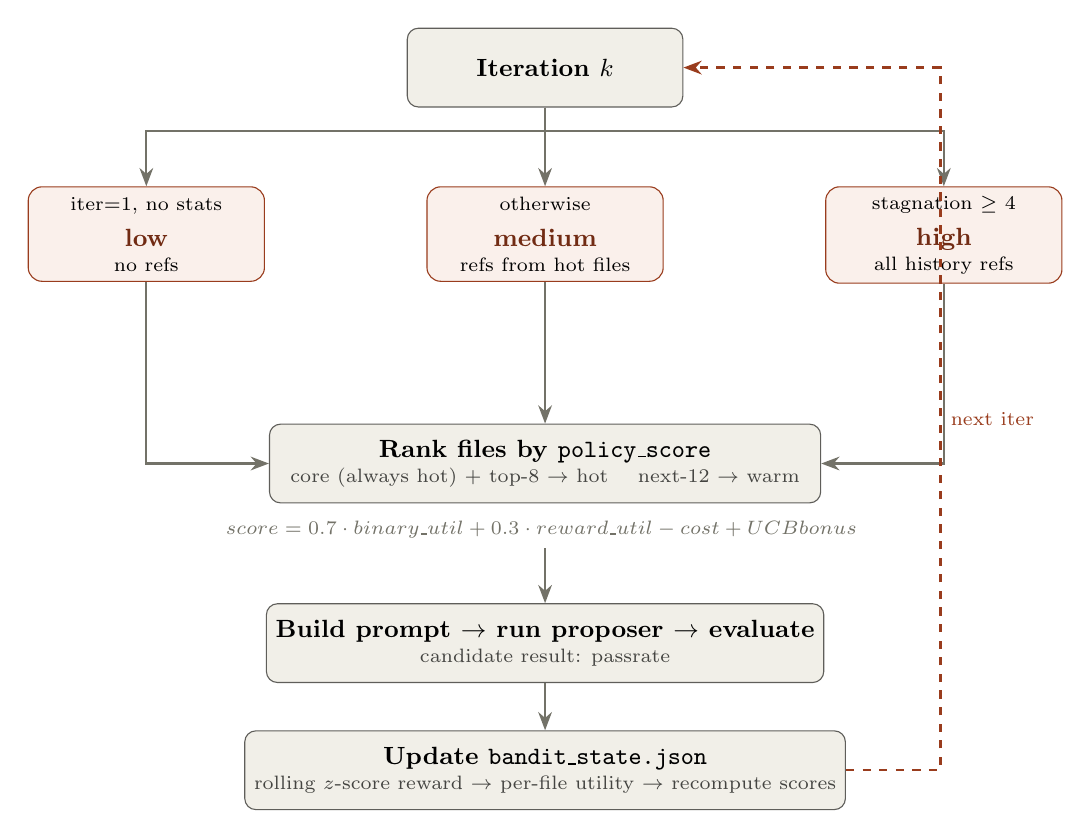
\begin{tikzpicture}[
    >=Stealth,
    node distance=0.7cm,
    every node/.style={font=\small},
    decision/.style={draw=decborder, fill=decfill, rounded corners=5pt,
        minimum height=1.2cm, minimum width=3.0cm, align=center},
    process/.style={draw=procborder, fill=procfill, rounded corners=4pt,
        minimum height=1.0cm, minimum width=7.0cm, align=center},
    arw/.style={->, thick, arrowgray},
    dasharw/.style={->, thick, dashed, feedbackcolor},
]

% Top entry
\node[process, minimum width=3.5cm] (entry) {\textbf{Iteration $k$}};

% Decision branches
\node[decision, below left=1.0cm and 1.8cm of entry] (d1) {
    {\scriptsize iter=1, no stats}\\[2pt]
    \textbf{\color{dectext}low}\\[-2pt]
    {\scriptsize no refs}
};
\node[decision, below=1.0cm of entry] (d2) {
    {\scriptsize otherwise}\\[2pt]
    \textbf{\color{dectext}medium}\\[-2pt]
    {\scriptsize refs from hot files}
};
\node[decision, below right=1.0cm and 1.8cm of entry] (d3) {
    {\scriptsize stagnation $\geq$ 4}\\[2pt]
    \textbf{\color{dectext}high}\\[-2pt]
    {\scriptsize all history refs}
};

\draw[arw] (entry.south) -- ++(0,-0.3) -| (d1.north);
\draw[arw] (entry.south) -- (d2.north);
\draw[arw] (entry.south) -- ++(0,-0.3) -| (d3.north);

% File ranking step
\node[process, below=1.8cm of d2] (rank) {
    \textbf{Rank files by \texttt{policy\_score}}\\[-2pt]
    {\scriptsize\color{proctext} core (always hot) + top-8 $\to$ hot \quad next-12 $\to$ warm}
};

\draw[arw] (d1.south) |- (rank.west);
\draw[arw] (d2.south) -- (rank.north);
\draw[arw] (d3.south) |- (rank.east);

% Scoring formula
\node[below=0.1cm of rank, font=\scriptsize\color{arrowgray}, align=center] (formula) {
    $\text{score} = 0.7 \cdot \text{binary\_util} + 0.3 \cdot \text{reward\_util} - \text{cost} + \text{UCB bonus}$
};

% Proposer
\node[process, below=0.7cm of formula] (proposer) {
    \textbf{Build prompt $\to$ run proposer $\to$ evaluate}\\[-2pt]
    {\scriptsize\color{proctext} candidate result: passrate}
};

\draw[arw] (formula.south) -- ++(0,-0.15) -- (proposer.north);

% Update state
\node[process, below=0.6cm of proposer, minimum width=5.0cm] (update) {
    \textbf{Update \texttt{bandit\_state.json}}\\[-2pt]
    {\scriptsize\color{proctext} rolling $z$-score reward $\to$ per-file utility $\to$ recompute scores}
};

\draw[arw] (proposer.south) -- (update.north);

% Feedback loop
\draw[dasharw] (update.east) -- ++(1.2,0) |- (entry.east)
    node[pos=0.25, right, font=\scriptsize\color{feedbackcolor}] {next iter};

\end{tikzpicture}
\end{document}
